\documentclass[12pt, twoside]{article}
\usepackage[letterpaper, margin=1in, headsep=0.5in]{geometry}
\usepackage[english]{babel}
\usepackage[utf8]{inputenc}
\usepackage{amsmath}
\usepackage{amsfonts}
\usepackage{amssymb}
\usepackage{tikz}
%\usetikzlibrary{quotes, angles}

\usepackage{graphicx}
\usepackage{enumitem}
\usepackage{multicol}

\usepackage{fancyhdr}
\pagestyle{fancy}
\fancyhf{}
\renewcommand{\headrulewidth}{0pt} % disable the underline of the header

\fancyhead[LE]{\thepage}
\fancyhead[RO]{\thepage \\ Name: \hspace{4cm} \,\\}
\fancyhead[LO]{BECA / Dr. Huson / Geometry\\* Prior knowledge assessment\\* 5 December 2019}

\begin{document}
\subsubsection*{0.1 Quiz: Slope, graphing linear equations}
  \begin{enumerate}

  \item Write down the slope and $y$-intercept of each linear equation.
  \begin{enumerate}
    \item $y=\frac{5}{2} x+9$. \\[1cm]
      slope: \hspace{6cm} $y$-intercept: \\[0.5cm]
    \item $y=-x+1$. \\[1cm]
      slope: \hspace{6cm} $y$-intercept: \\[0.5cm]
    \item $2x+2y=14$? \\[4cm]
      slope: \hspace{6cm} $y$-intercept: \\[0.5cm]
    \item $-2x+y=1$? \\[4cm]
      slope: \hspace{6cm} $y$-intercept: \\[0.5cm]
  \end{enumerate}

  \item What is the slope of a line parallel to the line $x-3y=15$?  
  \vspace{1.5cm}


\newpage
  \item Graph and label the two equations. Mark their intersection as an ordered pair.
    \begin{multicols}{2}
      $y = x+7$ \\
      $4x+5y=-10$
    \end{multicols}     \vspace{4cm}


    \begin{center} %4 quadrant regents grid w T-Chart
    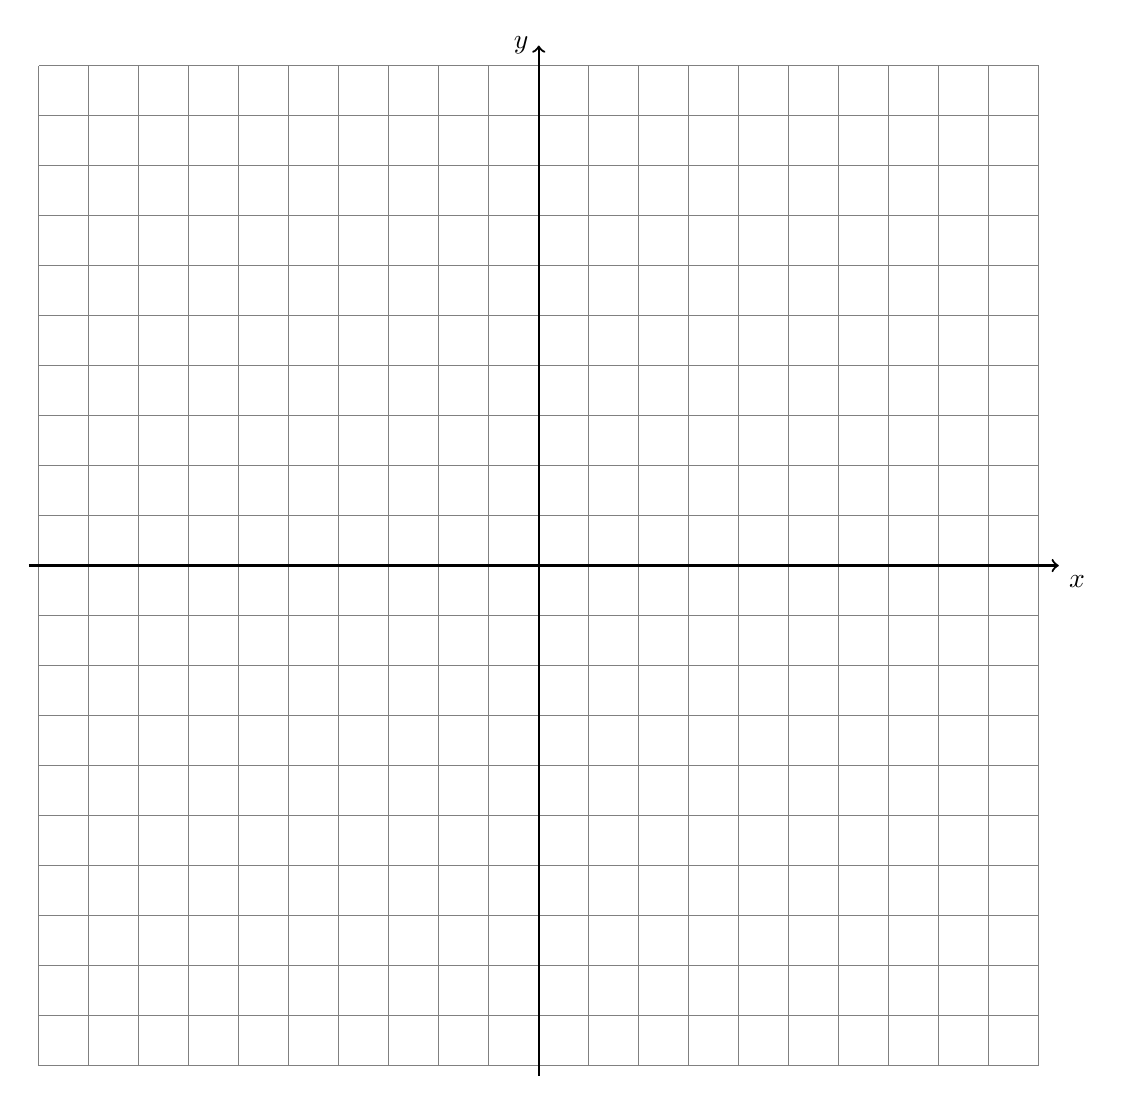
\begin{tikzpicture}[scale=.635]
      \draw [help lines] (-10,-10) grid (10,10);
      \draw [thick, ->] (-10.2,0) -- (10.4,0) node [below right] {$x$};
      \draw [thick, ->] (0,-10.2)--(0,10.4) node [left] {$y$};
    \end{tikzpicture}
    \end{center}

\end{enumerate}
\end{document}
